% ---------------------------------------------------------------------
% ---------------------------------------------------------------------
% ---------------------------------------------------------------------

\chapter{Experimentació i avaluació}
\label{cap05__}

% ---------------------------------------------------------------------
% ---------------------------------------------------------------------
% ---------------------------------------------------------------------

% Ací parlem de dades, partint de la tècnica del capítol Model Acústic
% Configuracions de param, resultats, etc 
% És un TFG, no un paper: podem/debem ser tiquismiquis i especificar el que cregam

En el present capítol es presenten aspectes tècnics i experimentals sobre el desenvolupament i optimització d'un sistema ASR de la llengua francesa, així com els resultats i les mètriques obtingudes a cada pas realitzat. El model acústic desenvolupat en aquest treball es combinarà amb diferents models del llenguatge desenvolupats per companys investigadors del MLLP-VRAIN i, finalment, es realitzarà una comparativa dels sistemes ASR resultants d'aquestes combinacions, amb un sistema ASR Francés desenvolupat a l'any 2017.

Aquest capítol s'estructura de la següent manera. En primer lloc, la Secció~\ref{cap05_software} descriu les ferramentes software utilitzades per al desenvolupament del model acústic.
En segon lloc, la Secció~\ref{cap05_prepro} exposa els passos duts a terme per preprocessar les dades.
A continuació, la Secció~\ref{cap05_am} descriu amb detall el procés d'entrenament dels diferents models acústics.
Després, la Secció~\ref{cap05_decod} detalla el procés d'optimització dels sistemes ASR resultants de la combinació dels diferents models acústics i de llenguatge considerats a aquest treball.
Per finalitzar, la Secció~\ref{cap05_aval} proporciona els resultats d'avaluació finals dels sistemes ASR proposats, així com del sistema de l'any 2017, realitzant un anàlisi comparatiu de les seves prestacions.

\section{Ferramentes software}
\label{cap05_software}
Durant la construcció del model acústic s'han emprat diferents ferramentes software, així com scripts per automatitzar les diferents tasques prèviament esmentades. D'aquestes destaquem principalment dues.

D'una banda s'ha emprat el software transLectures-UPV toolkit~\cite{tlk} (TLK), un toolkit que proveeix un conjunt de llibreries i ferramentes per a la construcció de sistemes ASR híbrids d'avantguarda.
Aquest software ha estat desenvolupat a l'UPV pel grup d'investigació MLLP-VRAIN, inicialment en el projecte transLectures~\cite{translectures} i que ha anat incorporant els últims avanços en tecnologia ASR híbrida. És capaç de preprocessar dades acústiques, entrenar models acústics, i descodificar senyals acústiques. En aquest cas, TLK s'ha utilitzat per al preprocessat de les dades, entrenar el model GMM-HMM, entrenar el model FF-DNN-HMM, calcular alineaments de senones a nivell de frame, i descodificar (reconèixer) automàticament dades de \textit{development} i \textit{test} per a la optimització i avaluació de sistemes ASR.
Per a assolir-ho, s'han gastat les següents ferramentes:
\begin{itemize}
    \item \texttt{tLextract}: s'encarrega de realitzar l'extracció de característiques dels fitxers indicats; rep com entrada una llista dels fitxers d'àudio i una llista dels fitxers d'eixida on s'escriuen les mostres (vectors de característiques).
    \item \texttt{tLtask-preprocess}: preprocessa fitxers multimèdia i transcripcions per a poder utilitzar-los amb TLK. Internament crida a \texttt{tLextract}.
    \item \texttt{tLtask-trainghmm}: realitza l'entrenament d'un model acústic GMM-HMM. Internament crida a múltiples scripts que s'encarreguen de realitzar tasques concretes de l'entrenament. Tots els paràmetres necessaris se li especifiquen des d'un fitxer de configuració.
    \item \texttt{tLdnn-train}: realitza l'entrenament d'un model acústic DNN-HMM. Tots els paràmetres necessaris se li especifiquen des d'un fitxer de configuració.
    \item \texttt{tLtask-align}: calcula l'alineament de senones a nivell de frame de les mostres que rep com a entrada. Tots els paràmetres necessaris se li especifiquen des d'un fitxer de configuració.
    \item \texttt{tLtask-recognise}: és la ferramenta utilitzada per a realitzar la descodificació de mostres (vectors de característiques). Rep com a entrada els models acústics i del llenguatge involucrats en el reconeixement, a més dels paràmetres propis.
\end{itemize}
    
    Per a l'entrenament de la xarxa del model BLSTM, s'ha utilitzat TensorFlow~\cite{tensorflow}, una biblioteca de codi obert desenvolupada per l'equip de Google Brain, destinada a la realització de tasques d'aprenentatge profund i automàtic.
    

\section{Preprocés de dades}
\label{cap05_prepro}

En la Secció~\ref{cap04_corpus} estan especificades les dades de parla transcrita que s'han utilitzat per entrenar i optimitzar els models acústics desenvolupats a aquest treball. No obstant això, aquests corpus necessiten passar per diversos passos de preprocès i d'extracció de característiques, descrits de manera conceptual a la Secció~\ref{cap03_prepro}, de cara a la seua homogeneïtzació i normalització abans de poder ser emprats per a entrenar els models.
Aquests passos es van realitzar amb l'eina \texttt{tLtask-preprocess}, de TLK, que internament crida a \texttt{tLextract}, encarregada de realitzar l'extracció de característiques segons els paràmetres que se li especifiquen.

El primer requisit que cal satisfer és que \texttt{tLextract} espera les dades acústiques amb unes característiques específiques: format d'àudio PCM (WAV) de 16 bits little endian, monocanal i amb una freqüència de mostreig de 16 KHz. 
La conversió es va realitzar amb l'eina \texttt{ffmpeg}, amb les opcions \texttt{-ac 1} i \texttt{-ar 16K} per a, respectivament, especificar l'eixida d'un únic canal i la freqüència de mostreig.
A l'eixida d'aquest pas vam obtindre les dades de tots els corpus en format WAV, monocanal i a 16 KHz.

A continuació es va emprar \texttt{tLtask-preprocess} dues vegades sobre cada corpus, per obtenir els dos tipus de vectors de característiques considerats a aquest treball:

\begin{itemize}
    \item MFCC: aquestos vectors de característiques es van generar amb 15 coeficients cepstrals i amb un coeficient extra per a l'energia del frame. També es van calcular la primera i segona derivada, que representen, respectivament, la velocitat i acceleració amb la que els seus valors canvien.
    Es van extraure vectors cada 10 ms, per poder emprar-los posteriorment amb finestres de context, i es normalitzen en mitjana i variància a nivell de vídeo/objecte. 
    D'aquesta manera, es van obtindre vectors de característiques de 48 components, que s'utilitzaren per entrenar els models de GMM-HMM i FF-DNN-HMM.

    \item Filterbanks: en aquest cas, s'empraren bancs de 85 filtres, sense derivades, resultant en vectors de característiques de 85 components amb els que es va entrenar el model BLSTM-HMM. 
\end{itemize}

Per acabar, es van preprocessar les transcripcions, açò és, eliminar signes de puntuació, convertir text a minúscules, transcriure dígits (conversió de xifres a paraules), entre altres tasques de normalització.
Primer vam desenvolupar i llançar un script que s'encarrega d'eliminar tots els signes de puntuació i convertir les majúscules a minúscules.
Finalment, s'analitzaren els resultats per a assegurar que no hi havia errors de preprocès. Es va utilitzar el llenguatge de programació de processament de text \texttt{awk}, junt a \texttt{sed}, la popular utilitat \textit{Unix} per a esmenar els problemes detectats als fitxers de transcripcions dels còrpora afectats. Aquest procediment es va repetir diverses vegades fins a trobar que el preprocès de les dades era correcte.



\section{Entrenament de models acústics}
\label{cap05_am}
En aquest treball hem considerat una topologia de models HMM estàndar en ASR, consistent en models de tres estats i estrictament linear, és a dir, un estat $q_t$ solament pot transicionar a ell mateix mitjançant un bucle, o a l'estat posterior $q_{t+1}$. Els fonemes es divideixen estructuralment en tres parts: transició del fonema previ (o silenci), part central, i part de transició al fonema posterior (o silenci). Aquestes tres parts estructurals són modelades seqüencialment per cadascun dels tres estats que componen els HMMs considerats a aquest treball.


\subsection{GMM-HMMs}
\label{cap05_am_gmm}
 
%%%%%%%%%%%%%%%%%%%%%%%%%%%
%%%
%%%   Entrenament GMM-HMM
%%%

Prèviament a realitzar l'entrenament del model GMM-HMM basat en mixtures de Gaussianes, cal generar un diccionari de pronunciacions fonètiques de les paraules presents a les transcripcions del conjunt \textit{train}. Aquest diccionari s'anomena \textit{lexicon} o model lèxic.
En aquest cas, emprarem un sistema estadístic de conversió de paraules a fonemes, anomenat Grapheme2Phoneme (G2P), amb un model pre-entrenat per a la llengua francesa, heretat del sistema ASR de l'any 2017, que rep com a entrada un fitxer amb tot el vocabulari de les dades de \textit{train}. Aquesta ferramenta genera el lexicon, amb les diferents transcripcions fonètiques possibles per a cadascuna de les paraules del vocabulari.
A continuació, es va realitzar una inspecció semi-automàtica del lexicon per depurar possibles errors de conversió fonètica.


L'entrenament dels models GMM-HMMs es va realitzar amb l'eina \texttt{tLtask-trainghmm}, que implementa l'algorisme Baum-Welch.
Com que l'entrenament es realitza en un clúster de computació distribuït d'altes prestacions, els fitxers necessaris per a l'entrenament es copiaren localment als nodes d'execució per minimitzar el coll de botella d'entrada-eixida a través de la xarxa mitjançant el protocol NFS (Network File System).
L'entrenament del model de monofonemes es va realitzar en 8 iteracions sobre totes les dades de \textit{train}, mentre que els models de trifonemes i trifonemes lligats basats en Gaussianes i mixtures de Gaussianes utilitzaren únicament 4 iteracions.

En aquest pas, TLK aplica automàticament l'algorisme CART. La configuració especificada per a la seua creació fou: una ocupació mínima per fulla de 2000 elements, un increment de la versemblança mínim per a continuar ramificant de 1500 punts.
Després d'aplicar l'algorisme CART amb aquesta configuració, vam obtenir 21589 estats nugats HMM o senones.
\texttt{tLtask-trainghmm} crea un fitxer que conte tots els trifonemes, agrupats per senones, anomenat \textit{tlist}.

%monofonemes -> 8 iteracions
%trifonemes  -> 4 iteracions
%trifo-tied  -> 4 iteracions
%mixtura de fins 64 components
%histogram pruning a 7500

En darrer lloc, vam entrenar, iterativament, els models trifonemes nugats amb mixtures de Gaussianes, sent un total de 7 models de $2^i : 0 \leq i \leq 7$ Gaussianes cada un. Aquest fou el procés més costós, ja que cada vegada que es duplicava el nombre de components, augmentava proporcionalment el temps de còmput. Com a mostra, el model de Gaussianes de 64 components va requerir 54 hores i 14 minuts de computació al clúster, emprant fins a 30 nuclis CPU Intel i7 en para\lgem el. 

Tot el procés d'entrenament dels models GMM-HMM ha requerit un temps d'execució de 4 dies, 14 hores i 49 minuts, emprant fins a 30 nuclis CPU Intel i7.
Per tal de validar la correcció d'aquest model acústic, vam construir un sistema ASR temporal, conformat per aquest model acústic i una taula de look-ahead derivada del model de llenguatge del sistema ASR Francés de 2017. Amb aquest sistema, vam reconéixer automàticament el conjunt de \textit{development}, obtenint uns WERs de 45.3\% al corpus de PM i 30.7\% al corpus de UB.
Tot i que aquests valors de WER són elevats, entren dins de les expectatives que es tenen d'aquests tipus de models generatius, d'acord amb coneixement previ del grup de recerca MLLP-VRAIN.
%A la figura~\ref{fig:gmm_wer}.

%\begin{figure}[!ht]
%    \centering
%    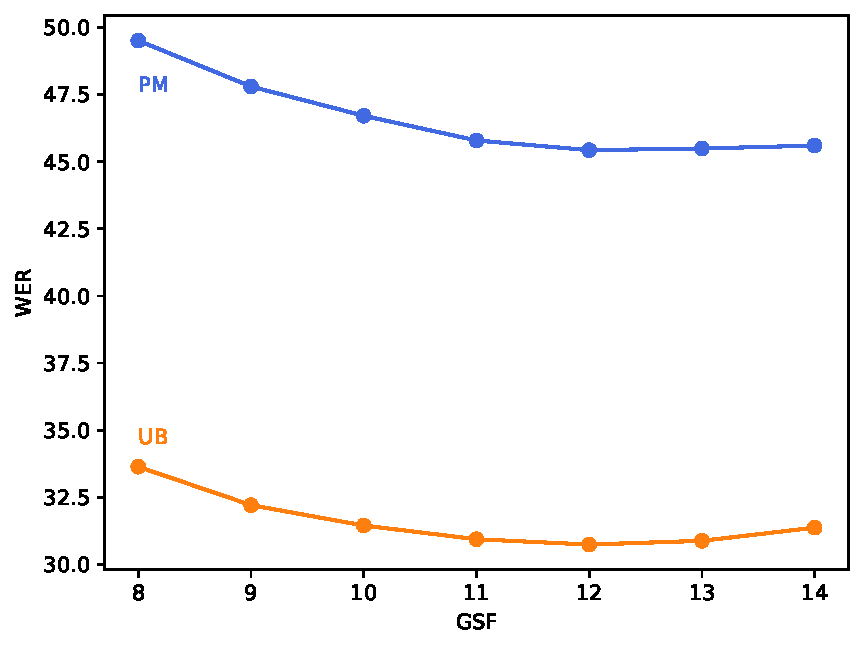
\includegraphics[width=0.5\textwidth]{figuras/gsf_gmm.pdf}
%    \caption{Resultats de l'exploració del valor GSF amb el model GMM-HMM i taules de look-ahead derivades del n-grama antic.}
%    \label{fig:gmm_wer}
%\end{figure}

%%%%%%%%%%%%%%%%%%%%%%%%%%%
%%%
%%%   Aliniament GMM-HMM
%%%

Finalment, vam usar l'eina \texttt{tLtask-align} amb el model GMM-HMM de 64 components, el \textit{lexicon}, la \textit{tlist}, els MFCCs i les transcripcions d'àudio per a obtenir els alineaments de senones a nivell de frame.
L'eina genera un fitxer d'eixida en el que s'indica, per a cada mostra d'entrenament, amb quins senones s'han alineat cadascun dels seus frames (vectors de característiques).




\subsection{FF-DNN-HMMs}
\label{cap05_am_dnn}
%%%%%%%%%%%%%%%%%%%%%%%%%%%
%%%
%%%   Entrenament DNN-HMM
%%%

El següent pas fou entrenar una FF-DNN per modelar $P(q_t|\textbf{x}_t)$ (veure Eq.~\ref{eq:cerca_nivell_paraules}) amb la informació dels alineaments calculats amb el model de GMMs. Per fer-ho, vam usar l'eina \texttt{tLdnn-train}. A continuació es detalla la configuració de la FF-DNN.
La capa d'entrada empra una finestra contextual de $\pm 5$ frames a esquerra i dreta del frame actual, es a dir, treballa amb vectors d'entrada de $11 \cdot 48 = 528$ components.
A continuació, sis capes ocultes de 2048 neurones amb activació per ReLu. Finalment, una capa d'eixida de 21589 unitats amb activació per softmax (tantes neurones com senones).
L'entrenament va requerir un temps d'execució total de 43 hores en una GeForce RTX 2080 Ti, al llarg de 20 èpoques, assolint un error de validació (FER) en \textit{development} de 56.1\%.
Si bé pot semblar una taxa d'error elevada, es tracta d'un valor acceptable, d'acord amb l'experiència  prèvia del grup MLLP-VRAIN. Alguns dels factors que justifiquen taxes FER elevades en aquest context són: en primer lloc, es tracta d'un problema de classificació complex, on hi ha que discriminar entre 21589 classes diferents. En segon lloc, les etiquetes de classe $q$ de totes les mostres d'entrenament, $(q, \textbf{x})$, proporcionades a la FF-DNN, han sigut generades per un model acústic generatiu, GMM-HMM, de baixes prestacions, pel que s'espera que una porció significativa de les etiquetes de classe siga incorrecta. Per últim, la funció d'error (FER) no considera l'existència d'etiquetes de classe (senones) similars. Per exemple, l'estat esquerre del trifonema \verb|l-a+o|, especialitzat en modelar la transició acústica del fonema \verb|/a/| al \verb|/l/|, i l'estat esquerre del trifonema \verb|k-a+o|, especialitzat en la transició del fonema \verb|/a/| al \verb|/k/|, són dues classes diferents, però pròximes entre elles i fàcilment confusibles. Però independentment del tipus d'error, FER sempre assigna error $= 1$ si l'etiqueta de classe no es exactament l'esperada, donant el mateix pes a errors greus que a errors assumibles.

Per tal de validar la correcció d'aquest model acústic, vam construir un segon sistema ASR temporal, conformat per aquest model acústic i la mateixa taula de look-ahead anterior. Amb aquest sistema, vam reconèixer automàticament el conjunt de \textit{development}, obtenint uns WERs de 29.0\% al corpus de PM i 23.0\% al corpus de UB.
Realitzant la comparació respecte al primer sistema, s'observa una millora notòria, assolint uns resultats potencialment prometedors. 

%\begin{figure}[!ht]
%    \centering
%    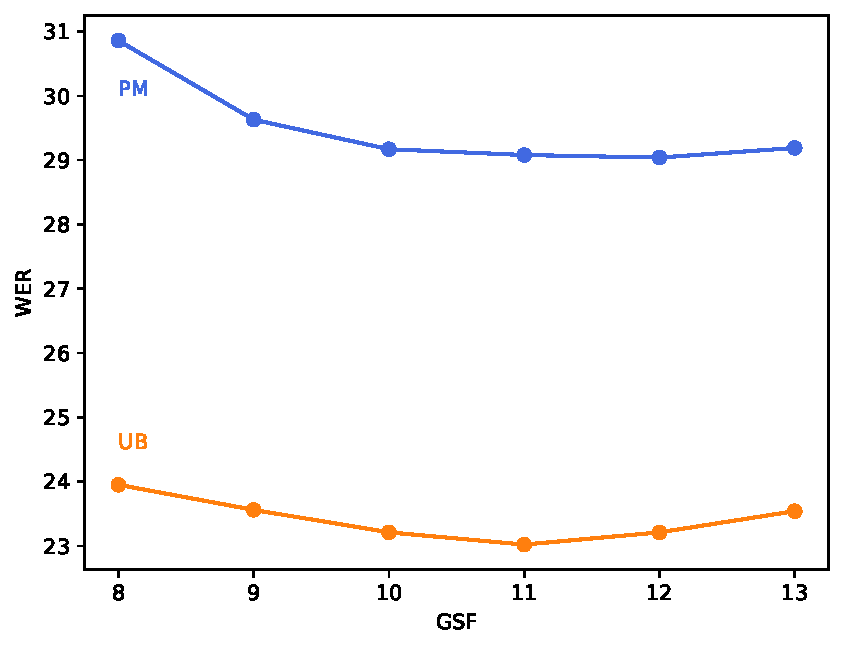
\includegraphics[width=0.5\textwidth]{figuras/gsf_dnn.pdf}
%    \caption{Resultats de l'exploració del valor GSF amb el model DNN-HMM i taules de look-ahead derivades del n-grama antic.}
%    \label{fig:dnn_wer}
%\end{figure}



%%%%%%%%%%%%%%%%%%%%%%%%%%%
%%%
%%%   Alineament DNN-HMM
%%%

Finalment, regenerarem els alineaments de senone a nivell de frame, usant la FF-DNN, amb l'objectiu d'obtenir una versió millorada d'aquests, similar a la millora observada en WER al conjunt de \textit{development} respecte al model GMM-HMM.




\subsection{BLSTM-HMMs}
\label{cap05_am_blstm}

%%%%%%%%%%%%%%%%%%%%%%%%%%%
%%%
%%%   Entrenament BLSTM-HMM
%%%

El pas final fou entrenar una xarxa BLSTM per modelar $P(q_t|\textbf{x}_t)$ amb la informació rebuda dels alineaments refinats, calculats pel model FF-DNN. Per fer-ho vam usar TensorFlow, mitjançant l'script \texttt{train\_blstm\_cudnn.py}. La configuració escollida de la BLSTM fou la següent.
S'utilitzaren 8 capes LSTM bidireccionals, cada una amb 512 neurones per a cada sentit temporal i, a l'igual com la FF-DNN, una capa d'eixida de 21589 neurones, tantes com senones.
Per a millorar la capacitat de generalització del model, es va aplicar la tècnica SpecAugment~\cite{park2019specaugment}, que consisteix en deformar les característiques d'entrada, emmascarar els blocs de canals de freqüència i emmascarar els blocs de passos de temps de forma aleatòria. Es realitzaren dues repeticions, amb màscares de 27 unitats d'ample horitzontal i 10 unitats d'ample vertical.

L'entrenament va requerir un temps d'execució total de 336 hores (aproximadament dues setmanes) emprant una GeForce RTX 1080, al llarg de 27 èpoques, assolint un error de validació (FER) mínim de 38.3\% sobre el conjunt de \textit{development}. La Figura~\ref{fig:wer_per_epoch} mostra l'evolució d'aquest error de validació en funció de les èpoques.
Comparant amb la FF-DNN, vam obtenir una reducció molt significativa del FER, de quasi 20 punts absoluts, demostrant, per una banda, la major capacitat d'aprenentatge d'aquest model, i d'altra banda, que els alineament refinats per la FF-DNN (les etiquetes de classe dels frames d'entrenament) són, efectivament, de major qualitat.

\begin{figure}[ht!]
    \centering
    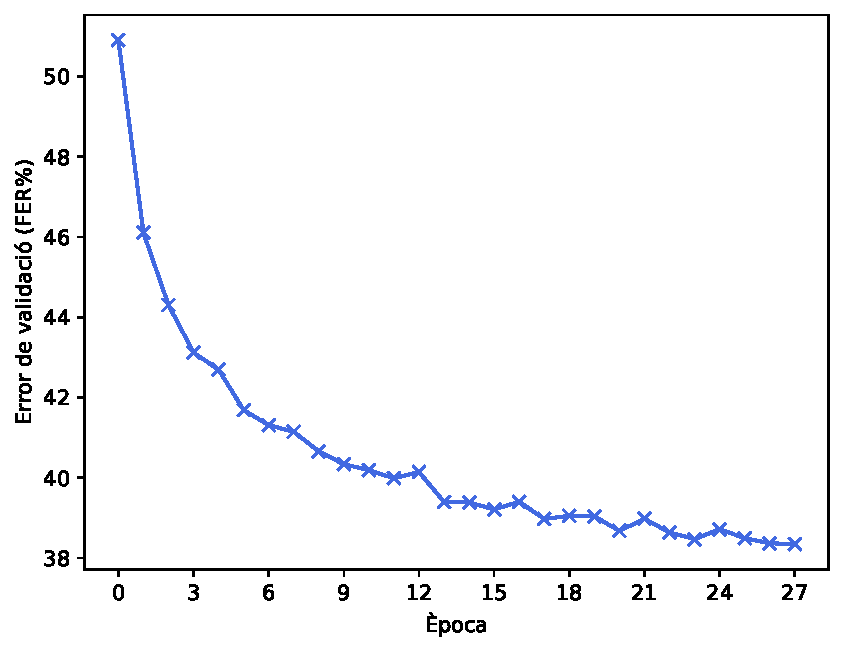
\includegraphics[width=0.6\textwidth]{figuras/validation_error.pdf}
    \caption{Error de validació en funció de les èpoques.}
    \label{fig:wer_per_epoch}
\end{figure}


\section{Construcció i optimització de sistemes ASR híbrids basats en BLSTM-HMM AMs}
\label{cap05_decod}
Una vegada entrenat el model acústic BLSTM-HMM, es procedeix a integrar-lo, juntament amb diferents models del llenguatge, en el descodificador híbrid de TLK per generar diferents sistemes ASR. Tots els LMs considerats en aquest treball han estat entrenats recentment per investigadors de l'MLLP, a excepció d'un model d'n-grames que prové del sistema ASR Francés de l'any 2017. A continuació es llisten i es donen els detalls més rellevants d'aquests LMs:

\begin{itemize}
    \item \textbf{n-grama (2017)}: model de 4-grames, provinent del sistema ASR Francés de 2017, entrenat amb totes les dades de text monolingüe descrites a la Secció~\ref{cap04_corpus_audio} (2.1G paraules), mitjançant el toolkit SRILM~\cite{srilm}. També es proporciona una versió superesporgada d'aquest model, convertida en taula estàtica de look-ahead per al descodificador.
    \item \textbf{n-grama}: model de 4-grames, entrenat amb totes les dades de text monolingüe (2.1G paraules), usant el toolkit KenLM~\cite{kenlm}. També es proporciona la taula estàtica de look-ahead corresponent.
    \item \textbf{TLM}: model de llenguatge neuronal basat en l'arquitectura Transformer, amb 24 capes Transformer, 512 neurones per capa, FF-DNNs de 4096 unitats, 12 \textit{attention heads}, i un \textit{embedding} de 768 dimensions, entrenat amb un subconjunt d'1G paraules amb el toolkit Fairseq~\cite{fairseq}.
    \item \textbf{n-grama + TLM}: interpolació lineal entre el 4-grama i el TLM, amb uns pesos òptims, calculats per al conjunt de development, de 40.7\% i 59.3\%, respectivament.
\end{itemize}

Per a la realització dels experiments, els valors dels LM look-ahead s'han calculat utilitzant un model molt esporgat derivat, en cada cas, del seu respectiu 4-grama. Al ser més menut, permet tindre precalculades totes les probabilitats en una taula i així accelerar la cerca. Així, quan en la cerca s'aplega a un node ``paraula'', la probabilitat d'aquest model menut es reemplaça per la del modl'original. Quan parlem d'emprar taules de look-ahead derivades d'un model, estarem parlant d'utilitzar directament les probabilitats d'aquest model esporgat.

Els sistemes ASR queden constituïts quan s'executa el descodificador de TLK mitjançant l'eina \texttt{tLtask-recognise}. Aquesta rep el model acústic (el model BLSTM-HMM), la taula de look-ahead estàtica, els vectors de característiques de les mostres a reconèixer i, opcionalment, un o més models del llenguatge externs, a banda dels valors dels diferents hiperparàmetres de descodificació.
D'aquests, destaquem els següents:

\begin{itemize}
    \item \textbf{GSF (Grammar Scale Factor)}, que escala el pes del model del llenguatge respecte al del model acústic durant la descodificació. 
    \item \textbf{PSF (Prior Scale Factor)}, que escala les probabilitats a priori, $P(q_t)$, dels HMM. 
    \item \textbf{LA (Grandària de la finestra, Look-Ahead)}, defineix el context futur, es a dir, el periode de temps, al que pot accedir la BLSTM per a buscar informació i emetre una possibilitat. És especialment útil quan tractem amb xarxes recurrents, ja que les permet considerar aquesta informació futura. Aquest paràmetre es necessari en un context d'streaming, ja que es la manera que tenim de limitar el futur necessari per a treballar.
    \item \textbf{LMHR (Language Model History Recombination)}, s'utilitza per a recombinar hipòtesis que utilitzen les mateixes últimes paraules a les seues histories. Força al descodificador a consolidar els prefixos de paraules i permetre una descodificació més ràpida, ja que la història del TLM no està limitada en longitud i ha de ser processada en cada iteració.
    \item \textbf{BEAM} representa la diferencia màxima que pot haver entre les puntuacions de l'objecte més probable i del menys probable. Així, si una hipòtesis es diferencia per un valor major al BEAM, es automàticament descartada. 
    \item \textbf{HP (Histogram pruning)}, defineix el nombre de històries màximes actives en cada instant.
    \item \textbf{LMHP (Language Model Histogram pruning)}, que controla el nombre d'històries noves que s'expandeixen a cada frame. Permet reduir el nombre de consultes al model del llenguatge.
\end{itemize}
En aquest cas, l'estudi dels paràmetres BEAM, HP i LMHP s'ha omès per restriccions temporals, sent valors fixes a BEAM$=160$, HP$=7500$ i LMHP$=60$, basats en coneixement previ del grup MLLP-VRAIN.

El primer sistema que vam estudiar utilitzava el model acústic BLSTM i les taules de look-ahead derivades del model d'n-grames de 2017.
Com que el LM era un cuatrigrama, l'LMHR no podia ser diferent de tres, en aquest i en posteriors experiments on sols intervé un 4-grama o una taula estàtica de look-ahead no es va explorar.
També s'ha estudiat l'impacte de la grandària de la finestra (lookahead), però no era significatiu, per tant, el seu valor va quedar fixat a $59$ frames al conjunt PM i $49$ frames al conjunt UB, tant en aquest com en posteriors experiments.
Finalment, es va estudiar el comportament davant de diferents valors del GSF i de PSF en funció del WER sobre el conjunt de \textit{development}. 
La Figura~\ref{fig:gsf_oldlm_small} mostra l'evolució del WER en funció del paràmetre GSF per a diferents valors de PSF.

\begin{figure}[ht!]
    \centering
    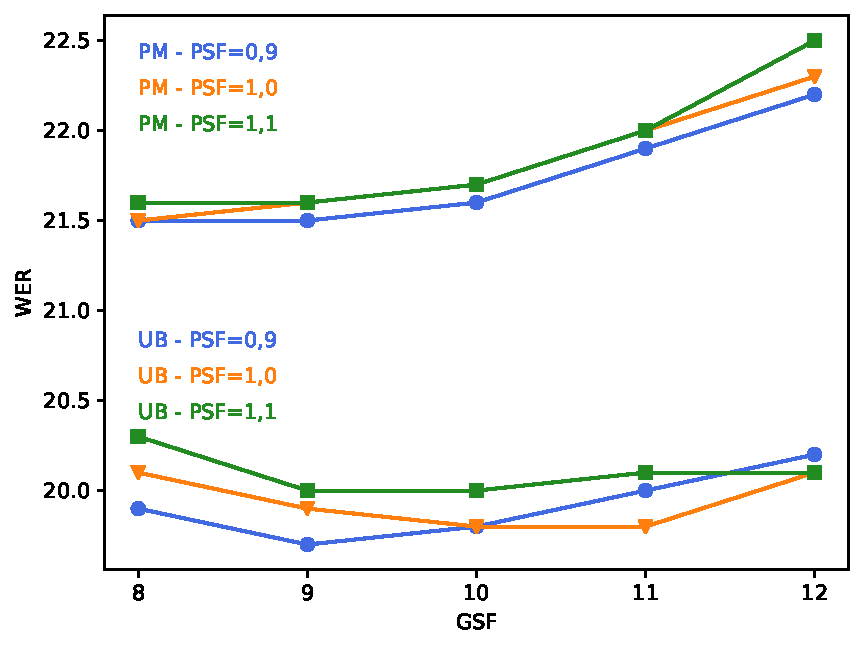
\includegraphics[width=0.5\textwidth]{figuras/gsf_oldlm_small.pdf}
    \caption{WER\%, calculat sobre els conjunts de \textit{development} de PM i UB, en funció dels paràmetres GSF i PSF amb el sistema format per el AM BLSTM i el LM basat en taules de look-ahead derivades del model del llenguatge de 2017. Es representen en diferents colors els valors de PSF per a ambdós corpus.}
    \label{fig:gsf_oldlm_small}
\end{figure}
Basant-se en les dades, el millor resultat per al conjunt PM, amb una WER de $21.5$\%, és el parell GSF=$8$ amb PSF= $1.0$ i GSF=$9$ amb PSF=$0.9$. Per a UB, el millor WER va ser $19.7$\%, per als valors de PSF=$0.9$ i GSF=$9$. Aquests valors de PSF van romandre fixos a la resta d'experiments, ja que no mostraven un gran impacte amb diferents valors.

En segon lloc, es va procedir a construir i optimitzar el sistema ASR resultant de combinar el nostre model acústic amb la taula de look-ahead estàtica i el LM de 4-grames de 2017.
En aquest cas es va optimitzar el GSF únicament, ja que el paràmetre LMHR encara necessitava estar fixat a tres.
La Figura~\ref{fig:gsf_oldlm_big} representa l'evolució del WER, calculat sobre els conjunts de \textit{development} de PM i UB, en funció del paràmetre GSF.

\begin{figure}[ht!]
    \centering
    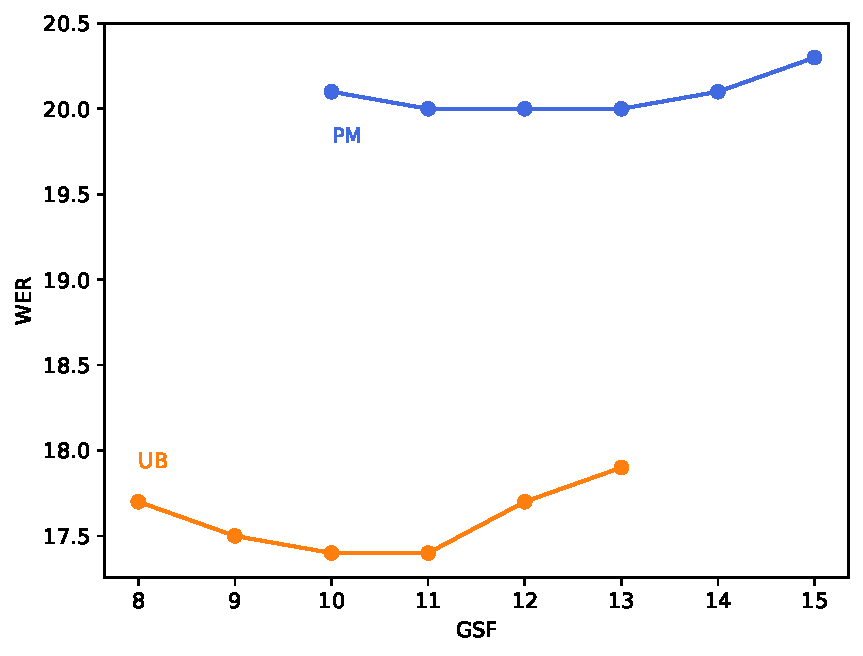
\includegraphics[width=0.5\textwidth]{figuras/gsf_oldlm_big.pdf}
    \caption{WER\%, calculat sobre els conjunts de \textit{development} de PM i UB, en funció del paràmetre GSF amb el sistema format pel AM BLSTM i el LM basat en taules de LA derivades del model del llenguatge de 2017 i el LM de 4-grames de 2017. Es representen en diferents colors els valors de PSF per a ambdós corpus.}
    \label{fig:gsf_oldlm_big}
\end{figure}
Obtinguérem unes puntuacions de WER de $20.5$\% per a PM, amb un GSF= $12$, i de $17.4$\% punts amb UB, amb un GSF=$10$. Veient aquests resultats es pot apreciar una millora respecte al model acústic antic, de $2$ punts de millora absoluta a PM i $0.9$ a UB.

En tercer lloc, estudiarem el comportament del nostre AM en conjunció dels nous LM de 4-grames.
En concret, vam portar a cap un primer experiment utilitzant sols la taula estàtica de look-ahead, i un segon que incorporava, a més, el model de 4-grames, explorant el GSF en cada cas.
La Figura~\ref{fig:gsf_newlm_sb} mostra els resultats d'ambdós experiments.

\begin{figure}[ht!]
    \centering
    \begin{subfigure}{0.45\textwidth}
        \centering
        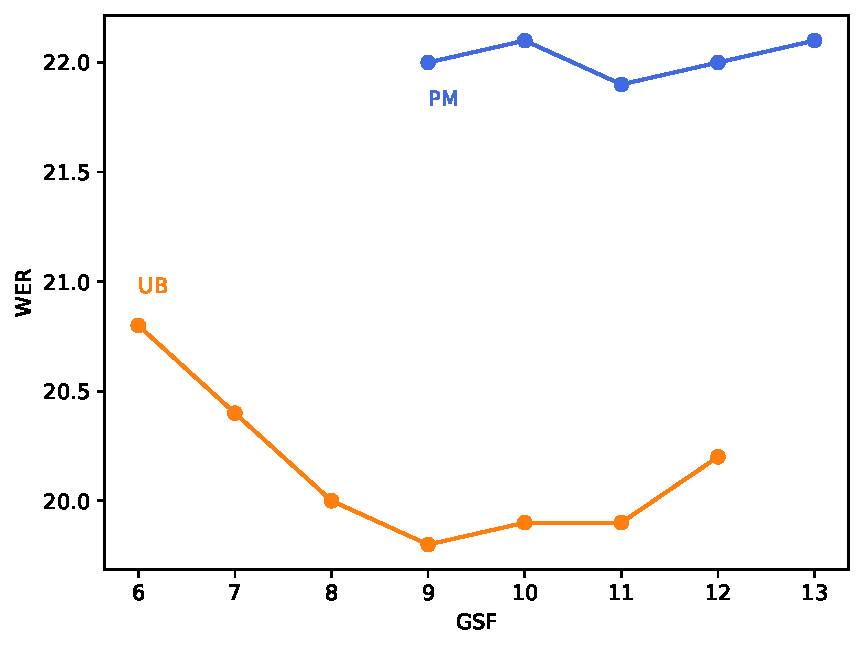
\includegraphics[width=\textwidth]{figuras/gsf_newlm_small.pdf}
        %\caption{Sistema amb taules de look-ahead basades en l'n-grama.}
    \end{subfigure}
    \begin{subfigure}{0.45\textwidth}
        \centering
        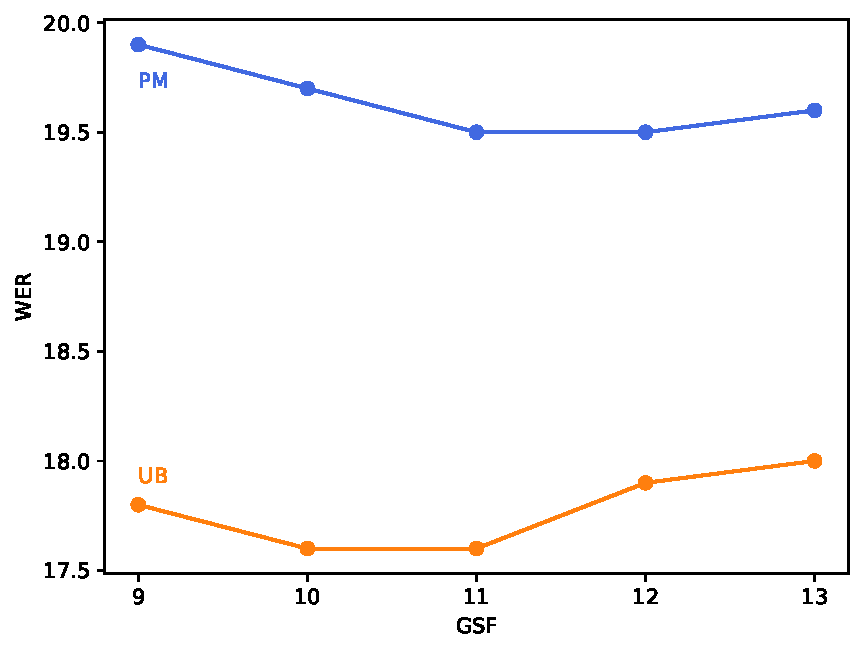
\includegraphics[width=\textwidth]{figuras/gsf_newlm_big.pdf}
        %\caption{Sistema amb taules de LA i l'n-grama nou.}
    \end{subfigure}
    \caption{WER\%, calculat sobre els conjunts de \textit{development} de PM i UB, en funció del paràmetre GSF; d'una banda (figura esquerra) per al sistema ASR que utilitza únicament les taules estàtiques de LA; i d'altra (figura dreta), per al sistema ASR que, a més, inclou el model de 4-grames.}
    \label{fig:gsf_newlm_sb}
\end{figure}

Pel que fa al model amb únicament taules de look-ahead, els millors resultats foren de $22.3$\% de WER a PM, amb GSF=$11$, i de $19.8$ punts a UB, amb GSF=$9$. Utilitzant també l'n-grama, les puntuacions milloraren fins a $20.1$\% en PM, amb GSF= $12$, i fins a $17.6$\% en UB, amb GSF= $11$.

En quart lloc, es va explorar la combinació del nostre AM amb el TLM. En un primer experiment fixarem el paràmetre LMHR $=9$ i explorarem els valors de GSF. La Figura~\ref{fig:gsf_newlm_tlm} mostra l'evolució del WER per als experiments, resultant que per a ambdós conjunts el millor valor fou GSF$=9$. Per aquesta raó, es va fixar a aquest valor i es va iniciar l'exploració de LMHR.

\begin{figure}[ht!]
    \centering
    \begin{subfigure}{0.45\textwidth}
        \centering
        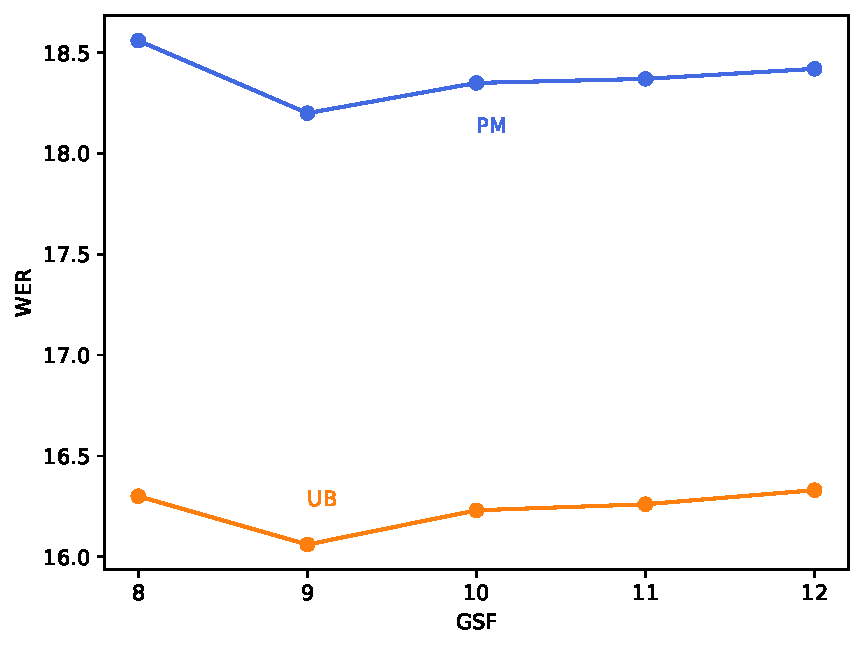
\includegraphics[width=\textwidth]{figuras/gsf_tlm.pdf}
    \end{subfigure}
    \begin{subfigure}{0.45\textwidth}
        \centering
        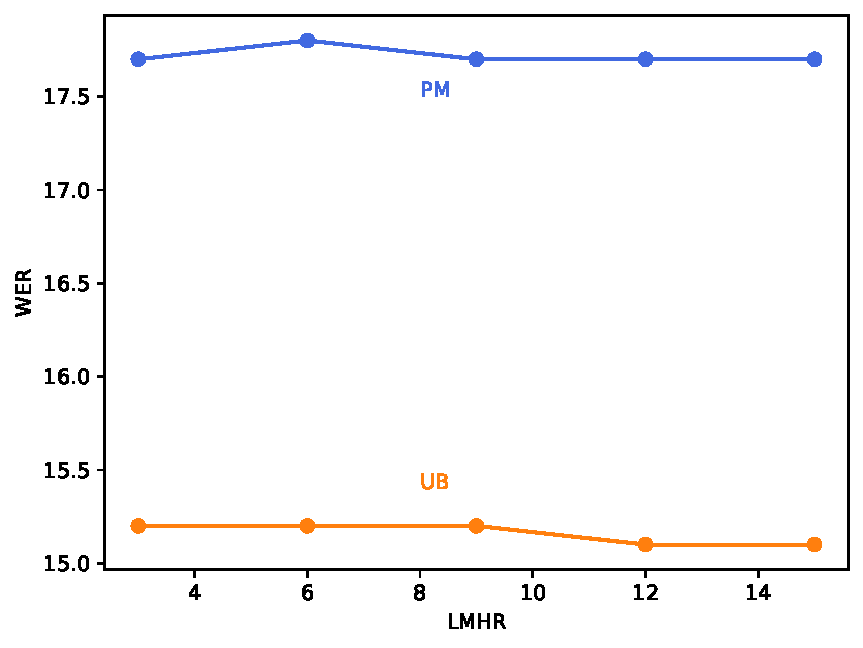
\includegraphics[width=\textwidth]{figuras/lmhr_tlm.pdf}
    \end{subfigure}
    \caption{}
    \caption{WER\%, calculat sobre els conjunts de \textit{development} de PM i UB per al sistema ASR que utilitza el TLM; d'una banda (figura esquerra) en funció del paràmetre GSF (fixant LMHR=3); i d'altra (figura dreta), en funció del paràmetre LMHR (fixant GSF=9).}
    \label{fig:gsf_newlm_tlm}
\end{figure}

Per una banda, s'obtingueren unes puntuacions WER de $18.4$\% per a PM, amb un LMHR de $9$, i de $16.0$\% per a UB, amb un LMHR de $9$. D'altra banda, el conjunt PM va obtindre una puntuació WER de $18.3$\% amb un LMHR de $6$, mentre que UB va obtindre una puntuació de $16.0$\% amb un LMHR de $12$.

Finalment, vam considerar el sistema que realitza una interpolació lineal entre l'n-grama i el TLM. El valor de LMHR va ser fixat al millor obtingut al pas anterior, ja que la mida mitjana de les frases al conjunt \textit{development} era d'aproximadament 10 paraules, i les variacions que podia aportar quedaven significantment reduïdes a costa del temps de còmput.
Els resultats poden observar-se a la Figura~\ref{fig:gsf_tlm_ngram}, aconseguint una WER en PM de $17.1$\% amb GSF$=11$, i de $15.2$\% amb GSF=$11$.

\begin{figure}[ht!]
    \centering
    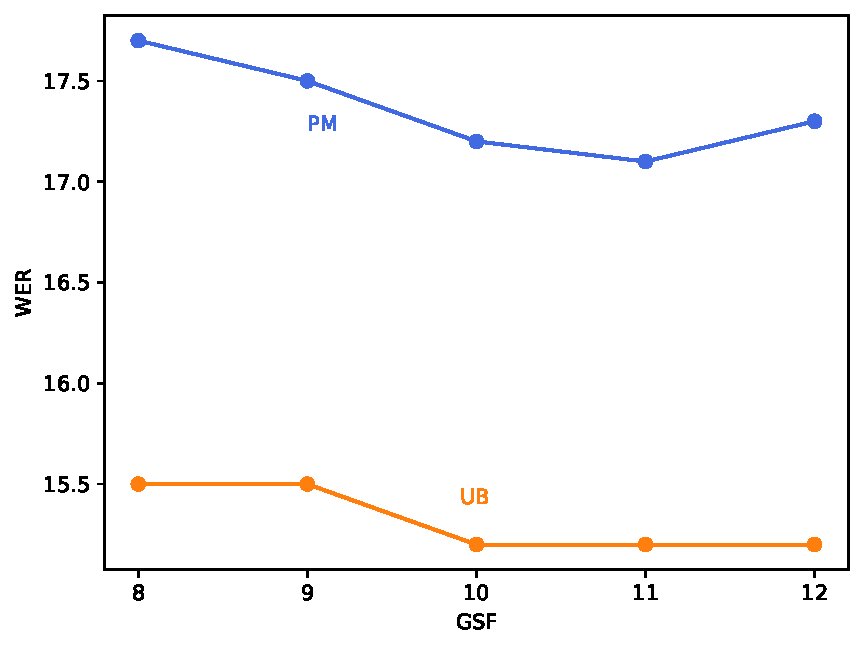
\includegraphics[width=0.5\textwidth]{figuras/gsf_tlm_ngram.pdf}
    \caption{WER\%, calculat sobre els conjunts de \textit{development} de PM i UB per al sistema ASR que utilitza l'interpolació lineal entre l'n-grama i el TLM en funció del paràmetre GSF.}
    \label{fig:gsf_tlm_ngram}
\end{figure}

\section{Avaluació i comparativa de sistemes ASR}
\label{cap05_aval}
En aquesta secció, primerament, es realitzarà l'avaluació final de tots els sistemes ASR considerats en el present treball, utilitzant els conjunts de \textit{test} de PM i UB. Després, els resultats de cada sistema es comparen amb els del sistema ASR Francés de 2017, per tal de mesurar l'efecte de les millores tecnològiques introduïdes.

El sistema ASR Francés de 2017 (d'ara endavant, sistema \textit{baseline}), és un sistema híbrid format per un model acústic FF-DNN-HMM amb activacions per ReLu, similar al model descrit al Capítol~\ref{cap03_dnnhmm}.
Aquest realitza, inicialment, un pas previ \guillemotleft Voice Activity Detection\guillemotright, que bàsicament es tracta de realitzar una segmentació d'on hi ha parla humana i on no per a únicament descodificar en aquests segments.
El procés de descodificació es realitza en dos passos. Un primer pas de reconeixement estàndard, i un segon pas amb \textit{fCMLLR (feature Constrained Maximum Likelihood Linear Regression)}, una tècnica que realitza una adaptació dels vectors de característiques a les locutores presents en les mostres, emprant les transcripcions automàtiques del primer pas de reconeixement com a referència.
Finalment, es realitza un tercer pas addicional, on és repuntuen les probabilitats del model del llenguatge amb un o diversos models del llenguatge externs més potents, en aquest cas, un 4-grama usat en els experiments de la Secció~\ref{cap05_decod}, i un model del llenguatge basat en RNNs.
El principal inconvenient d'aquest sistema és que, al ser multipassada, no està preparat per al reconeixement en streaming.
%Aquest sistema tenia les següents puntuacions WER: 22.1 i 19.0 punts per als corpus PM i UB al set \textit{dev} i 24.1 i 16.5 punts WER per als mateixos corpus al set \textit{test}.

Per altra banda, els sistemes ASR avaluats en aquest treball són aquells que acoblen el model BLSTM-HMM, amb la taula de look-ahead derivada del nou model d'n-grames, i diferents combinacions de models del llenguatge externs: 4-grama (2017), 4-grama, TLM i TLM interpolat amb 4-grama.
La taula~\ref{tab:resum_wer} resumeix les resultats WER, calculats sobre els conjunts de \textit{test} de PM i UB, amb tots els sistemes considerats en aquest estudi comparatiu.
També s'inclouen els millors resultats d'aquests sistemes en els respectius conjunts de \textit{development} (veure Secció~\ref{cap05_decod}).
%Les millores relatives del sistema BLSTM amb n-grama i Transformer respecte al sistema Baseline de 2017 són del 22.8\% al corpus de PM i del 15.6\% al corpus de UB.

\begin{table}[ht!]
    \centering
    \caption{WER\% dels diferents sistemes considerats en aquest estudi comparatiu, calculats sobre els conjunts de \textit{development} i \textit{test} dels corpus PM i UB. Els nostres sistemes estan representats de tal forma que els diferents LM proporcionats pel MLLP-VRAIN es combinen amb el AM desenvolupat en aquest treball.}
    \begin{tabular}{l|rr|rr}
                             & \multicolumn{2}{c|}{PM} & \multicolumn{2}{c}{UB} \\
        Sistema              & Dev        & Test       & Dev        & Test      \\ \hline
        Baseline (2017) & 22.1       & 24.1       & 19.1       & 17.3      \\
        BLSTM (+ taula LA)               & 22.3       & 22.2       & 20.7       & 19.0      \\
        \quad + n-grama (2017)       & 20.5       & 20.7       & 18.2       & 17.6      \\
        \quad + n-grama            & 20.1       & 20.2       & 18.4       & 17.4      \\
        \quad + TLM                & 17.7       & 18.9       & \textbf{15.1}       & 14.9      \\
        \qquad + n-grama  & \textbf{17.1} & \textbf{18.6} & 15.2  & \textbf{14.6}     
    \end{tabular}
    \label{tab:resum_wer}
\end{table}

Com pot observar-se, el sistema baseline és superat per tots els nostres sistemes ASR, excepte pel que únicament utilitza les taules de look-ahead, on obté un resultat pitjor en UB, però un poc millor en PM. Convé remarcar que el sistema de 2017 és un sistema multipassada que no està preparat per a funcionar en streaming. En canvi, els nous sistemes poden fer-ho.

També són rellevants les millores màximes, i és que quan es considera el TLM, s'obtenen unes millores absolutes de WER de fins a 5.5 punts, amb unes millores relatives del $22.8\%$ a PM i del $15.6\%$ a UB.

D'altra banda, convé ressaltar la comparativa entre el sistema baseline i el sistema BLSTM amb l'n-grama de 2017, ja que ens permet aproximar la millora que aporta el nostre model acústic al sistema final, a pesar que el sistema vell utilitzava un RNNLM que el nostre sistema no. Inclòs en aquest cas, s'assoleix una millora de les prestacions global, que arriba fins als 3.4 punts de diferència en el \textit{test} de PM, excepte en el \textit{test} d'UB, on el nostre sistema és lleugerament inferior en prestacions ($0.3$ punts WER). La nostra hipòtesi és que, en aquest cas concret, el model RNNLM marca la diferència, ajudant al sistema baseline a superar el nostre sistema.
